\section{The variance-reduced calibrator}
\label{sec:calibrating_models}

In the previous section we saw that the problem with scaling methods is we cannot estimate their calibration error. The upside of scaling methods is that if the function family is well suited \pl{can we be precise/short?} to the data they require $O(1/\epsilon^2)$ samples to reach calibration error $\epsilon$, while histogram binning requires $O(B/\epsilon^2)$ samples where $B$ can be large. Can we get a method that is sample efficient to calibrate and one where it's possible to estimate the calibration error? To achieve this\pl{,} we propose the variance-reduced calibrator (Figure~\ref{fig:var_red_binning}) where we first fit a scaling function, and then bin the outputs of the scaling function. Note that in previous work binning the outputs of a function was used for evaluation whereas here it is used for the method itself.

\subsection{Variance-reduced recalibration algorithm}

We split the recalibration data $T$ of size $n$ into 3 sets: $T_1$, $T_2$, $T_3$. The variance-reduced recalibration algorithm, illustrated in Figure~\ref{fig:variance_reduced_illustration}, outputs $\hat{g_{\mathcal{B}}}$ such that $\hat{g_{\mathcal{B}}} \circ f$ has low calibration error:

\textbf{Step 1 (Function fitting):} The first step is to select $g = \argmin_{g \in G} \sum_{(z, y) \in T_1} (y - g(z))^2$.
\pl{this should have been defined when you introduce Platt scaling}

\textbf{Step 2 (Bin construction):} The second step is to construct a suitable binning scheme. We choose the bins so that an equal number of $g(z_i)$ in $T_2$ land in each bin $I_j$ for each $j \in \{1, \dots, B\}$.
\pl{emphasize this is not evenly spaced bins like previous work}

\textbf{Step 3 (Discretization):} The third step is to discretize $g$, by outputting the average $g$ value in each bin---these are the gray circles in Figure~\ref{fig:var_red_binning}. Let $\mu(S) = \frac{1}{|S|} \sum_{s \in S} s$ denote the mean of a set of values.
Let $\hat{\mu}[j] = \mu(\{ g(z_i) \; | \; g(z_i) \in I_j \wedge (z_i, y_i) \in T_3 \})$ be the mean of the $g(z_i)$ values that landed in the $j$-th bin.
Then we set $\hat{g_{\mathcal{B}}}(z) = \hat{\mu}[\beta(g(z))]$ -- that is we simply output the mean value in the bin that $g(z)$ falls in.

\pl{why is $g$ not hatted and $\hat{g_\mathcal{B}}$ hatted? make consistent}

\pl{this is the key part of your method; generally, I'd try to move as much out that's not new to existing work and highlight what's new in what you're doing}
\ak{I tried to move out Platt scaling and binning to the setup, but I'd prefer having this here for completeness? I made step 1 and 2 much shorter than before.}
\pl{this is fine}

\subsection{Analysis}

We \pl{now} show that the variance-reduced calibrator requires $O(B + 1/\epsilon^2)$ samples to calibrate, and in the next section \pl{actually reference it} we show that we can efficiently measure its calibration error. For the main theorem, we make some standard regularity assumptions on $\mathcal{G}$ (Lipschitz, injectivity, bounded parameters) which we formalize in Appendix~\ref{sec:calibrating_models_appendix}. These hold for Platt scaling, Beta calibration~\cite{kull2017sigmoids}, and vector scaling. Our result is a generalization result---we show that if $\mathcal{G}$ contains \pl{some} $g^*$ with low calibration error, then our method will quickly find $\hat{g}_{\mathcal{B}}$ with low calibration error:

\begin{restatable}[Calibration bound]{theorem}{finalCalib}
\label{thm:final-calib}
Suppose that $\min_{g \in \mathcal{G}}\ell_2^2\mbox{-CE}(g) \leq \epsilon^2$.
  With $n = \widetilde{O}(B + \frac{d'}{\epsilon^2})$ samples, where $\widetilde{\Theta}$ hides log factors, the variance-reduced calibration algorithm \pl{estimator} finds $\hat{g}_{\mathcal{B}}$ with $\ell_2^2\mbox{-CE}(\hat{g}_{\mathcal{B}}) \leq 2 \epsilon^2$. Note that $d'$ is the number of parameters which is $1$ for Platt scaling.
\end{restatable}

We present a proof in Appendix~\ref{sec:calibrating_models_appendix} but give a sketch here. Step 1 of our algorithm, essentially \pl{isn't it exactly?} Platt scaling, simply fits a function $g$ to the data---standard statistical learning theory results show that $g$ converges in $O(\frac{1}{\epsilon^2})$ samples.

Step 3, where we bin the outputs of $g$, is the main variance-reduction step. If we had infinite data, Proposition~\ref{prop:bin_low_bound} showed that the binned version $g_{\bins{}}$ has lower calibration error than $g$, so we would be done. However we do not have infinite data---the core of our proof is to show that the empirically binned $\hat{g_{\bins{}}}$ converges to $g_{\bins{}}$ in $O(B + \frac{1}{\epsilon^2})$ samples, instead of $O(B + \frac{B}{\epsilon^2})$ samples in histogram binning. The intuition is in Figure~\ref{fig:variance_reduced_illustration}---the $g(z_i)$ values in each bin (gray circles in Figure~\ref{fig:var_red_binning}) are in a narrower range than the $y_i$ values (black crosses in Figure~\ref{fig:hist_binning}) so when we take the average\pl{,} we incur less of an estimation error\pl{less estimation error}. The perhaps surprising part is that this leads to a provably smaller dependency on the number of bins $B$ \pl{I think the surprising part is that we are estimating $B$ numbers with $1/\epsilon^2$ samples!}. In fact, there may be a small number of bins where the $g(z_i)$ values are not in a narrow range, but our proof still shows that the overall estimation error is small.

In Section~\ref{sec:challenges-measuring} we showed that we cannot measure the calibration error of scaling methods, in contrast we show that we \emph{can} measure the calibration error of our calibrator. Recall that we chose our bins so that each bin had an equal proportion of points---in order to estimate calibration error efficiently (Theorem~\ref{thm:final-ours}), we will require that this property approximately holds in the population as well.

\begin{definition}[Well-balanced binning]
Given a binning scheme $\mathcal{B}$ of size $B$, and $\alpha \leq 1$. We say $\mathcal{B}$ is $\alpha$-well-balanced if for all $j$,
  \[ \frac{1}{\alpha B} \leq \pl{\mathbb P} P(Z \in I_j) \leq \frac{\alpha}{B}\]
\end{definition}

\begin{lemma}
\label{lem:well-balanced}
If $n \geq B\log{\frac{B}{\delta}}$, with probability at least $1 - \delta$, the binning scheme $\mathcal{B}$ we chose is 2-well-balanced.
\end{lemma}

While the way we choose bins is not novel \pl{cite; this is important because earlier we say that most people choose equally sized bins...probably should mention this binning strategy too then}, we believe the guarantees around it are---not all binning schemes in the literature allow us to efficiently estimate the calibration error, for example the binning scheme in~\cite{guo2017calibration} does not. Our proof of Lemma~\ref{lem:well-balanced} is in Appendix~\ref{sec:calibrating_models_appendix}. The core challenge is that applying Chernoff bounds or \pl{and? I think of these as complementary} a standard VC dimension argument gives us a loose bound and tells us we need $O(B^2\log{\frac{B}{\delta}})$ samples. We use a discretization argument to prove the result.

In Proposition~\ref{prop:mse-finite-binning} in Appendix~\ref{sec:calibrating_models_appendix}, we also show that if we use lots of \pl{many} bins, binning the outputs has little impact on model quality as measured by the mean-squared error.


\pl{I didn't find this section that satisfying;
first we should move stuff about scaling and binning out of this section and start this section by saying can we combine the best of the two worlds and mention $O(B + 1/\epsilon^2)$ - this is easy;
Then the big thing that's missing is the insight into why the proposed algorithm works and how the analysis proceeds,
kind of like a proof sketch
}
\ak{I've edited it a lot, is it looking better?}
\pl{yes!}

\subsection{Experiments}

Our experiments on CIFAR-10 and ImageNet show that in the low-data regime, for example when we use $\leq 1000$ data points to recalibrate, our variance-reduced calibration method produces models with much lower calibration error than histogram binning. The model's objective was to output a confidence score associated with each class, where we calibrated each class separately as in~\cite{zadrozny2002transforming}, used $B$ bins per class and evaluated calibration using the marginal calibration error (Definition~\ref{dfn:marginal-ce}).

We describe our experimental protocol for CIFAR-10.
The CIFAR-10 validation set has 10,000 data points. We sampled, with replacement, a recalibration set of 1,000 points. We ran either the variance-reduced calibrator (we fit a sigmoid in the function fitting step) or histogram binning and measured the marginal calibration error on the entire set of 10K points.
% \footnote{This is equivalent to using the empirical distribution on the 10K validation points as the true data distribution, and comparing how these methods perform. We do this since we cannot measure the ground truth calibration error.}
We repeated this entire procedure 100 times and computed mean and 90\% confidence intervals, and we repeated this varying the number of bins $B$. Figure~\ref{fig:marginal_calibrator_comparison_cifar} shows that the variance reduced calibrator produces models with lower calibration error, for example $35\%$ lower calibration error when we use 100 bins per class.

Using more bins allows a model to produce more fine-grained predictions e.g.~\cite{brocker2012empirical} use $B = 51$ bins. This improves the quality of predictions which can be measured by the mean-squared error -- Figure~\ref{fig:cifar_calibrator_cmp_mse_ce} shows that our method achieves better mean-squared errors for any given calibration constraint. More concretely, the figure shows a scatter plot of the mean-squared error and $\ell_2^2$ calibration error for histogram binning and variance-reduced calibration when we vary the number of bins. For example, if we want our models to have an $\ell_2^2$ calibration error $\leq 0.0004$ (which translates to an $\ell_2$ `average' calibration error of 2\%) we get a $10\%$ better mean-squared error. In Appendix~\ref{sec:calibrating_models_appendix_experiments} we give more experiment details and we show that these results hold for top-label calibration and for ImageNet.
% We also run an ablation to show that if we have more data points then as the theory predicts histogram binning catches up to the variance-reduced calibrator, and that the way we construct bins is crucial, the result do not hold if we use the binning scheme in~\cite{guo2017calibration}.

\begin{figure}
  \centering
  \centering
     \begin{subfigure}[b]{0.55\textwidth}
         \centering
         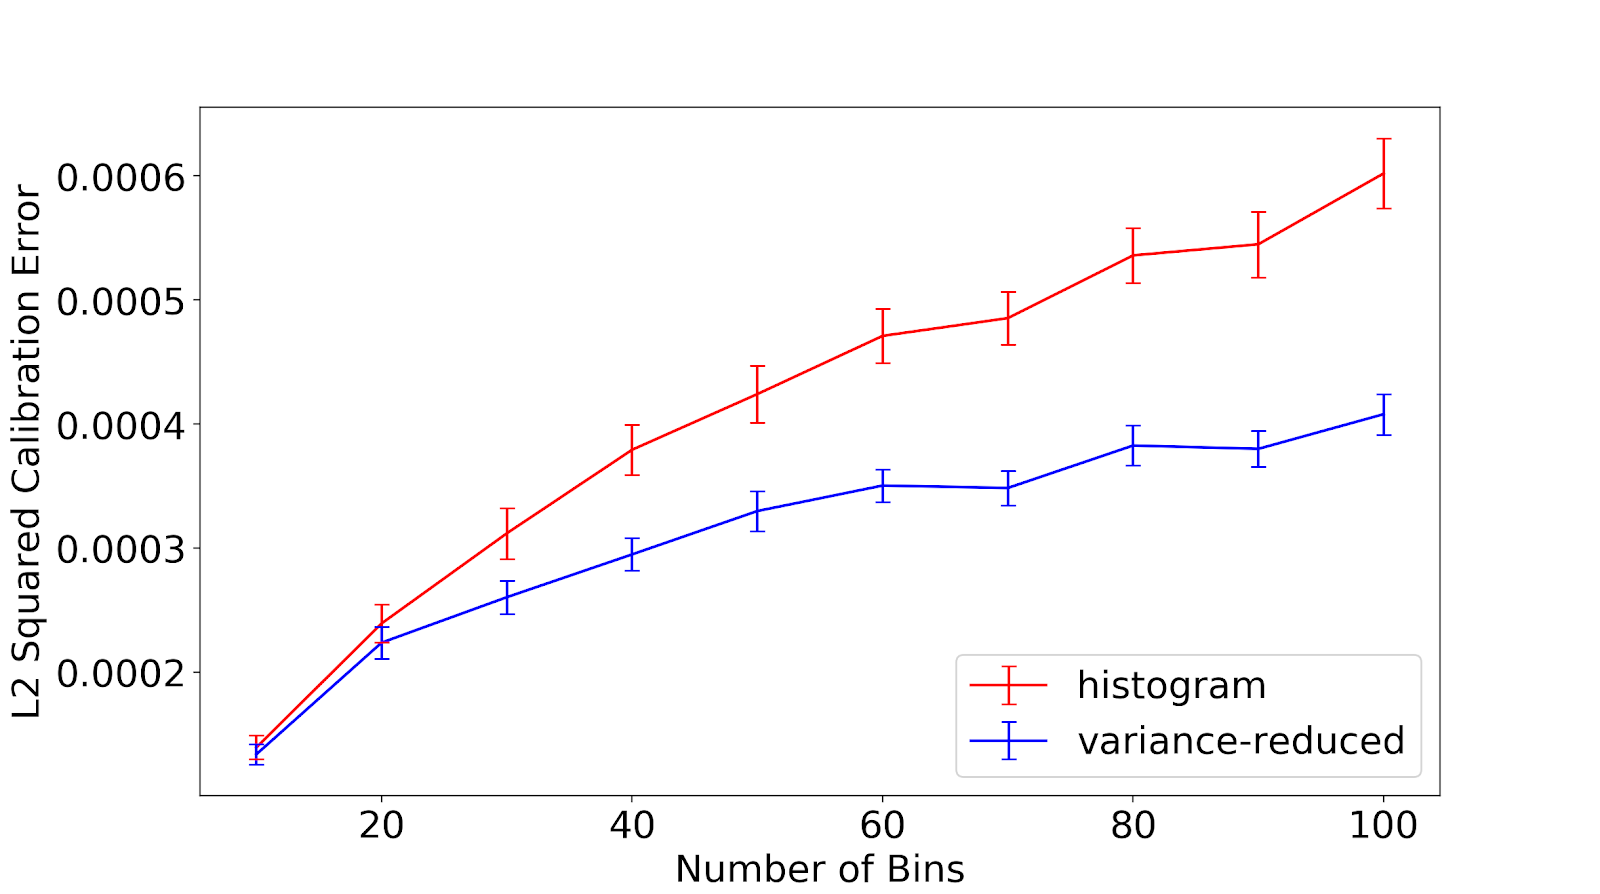
\includegraphics[width=\textwidth]{marginal_cifar_hist_vs_ours_bins.png}
         \caption{$\ell_2^2$ calibration error vs $B$. \pl{Effect on number of bins}}
         \label{fig:marginal_calibrator_comparison_cifar}
     \end{subfigure}
     \hfill
     \begin{subfigure}[b]{0.4\textwidth}
         \centering
         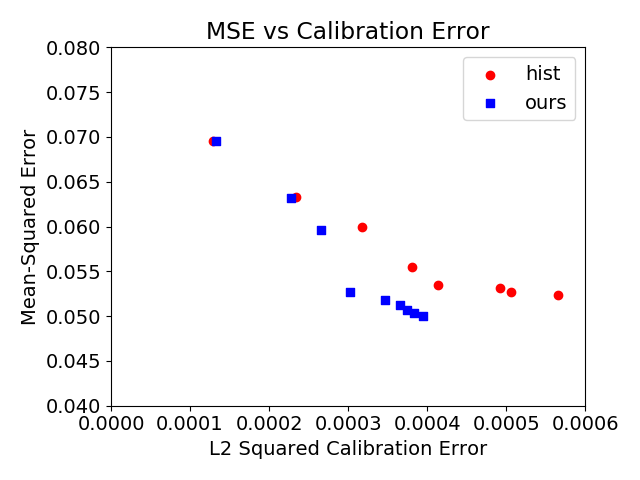
\includegraphics[width=\textwidth]{mse_vs_ce_calibrators_cifar.png}
         \caption{MSE vs $\ell_2^2$ calibration error. \pl{Tradeoff between calibration and MSE}}
         \label{fig:cifar_calibrator_cmp_mse_ce}
     \end{subfigure}
  \caption{
  (\textbf{Left}) Recalibrating using 1,000 data points on CIFAR-10, our variance-reduced calibrator achieves lower $\ell_2^2$ calibration error than histogram binning, especially when the number of bins $B$ is large.
  (\textbf{Right}) For a fixed calibration error, our variance-reduced calibrator allows us to use more bins. This results in models with more predictive power which can be measured by the mean-squared error. Note the Y-axis range is $[0.4, 0.8]$ to zoom into the relevant region.
  \pl{change legend to 'histogram binning' and variance-reduced estimator' for both for consistency}
  \tm{if we have time, we could also make the x,y lablel font bigger. and use scientific formt for xtick and ytick; and maybe slightly bigger legend.}
  }
  \label{fig:nan2}
\end{figure}



% Our experiments suggest that the binned calibration error gives us a poor sense of a model's calibration error if the model outputs a continuous range of values.
% We now turn to the question of how to produce models that we can \emph{verify} are calibrated.
% We describe \pl{propose} the \pl{the 'the' is bothering me a bit now that I keep on seeing it; strikes me as a bit presumptuous
% because it's like you're implicitly claiming that your estimator is the only one that reduces variance} variance-reduced calibrator (Figure~\ref{fig:variance_reduced_illustration}), and prove bounds on its sample complexity.
% In particular, assuming the function family $\mathcal{G}$ \pl{where did $\mathcal{G}$ come from? came out of nowhere} is well suited to recalibrate the data, we require $O(\frac{1}{\epsilon^2})$ samples to achieve calibration error $\epsilon$, while histogram binning requires $O(\frac{B}{\epsilon^2})$ samples.
% Moreover, unlike methods such as Platt scaling and temperature scaling, we can then check if our model is calibrated (see Section~\ref{sec:verifying_calibration}).
% If the model is not calibrated we can, for example, try different families $\mathcal{G}$ or collect more data and use histogram binning.
% \pl{I feel like this is getting too confusing;
% I'd just keep the story simple:
% begin by summarizing, in the previous section, we saw scaling techniques which are great because they are parametric, requiring only $O(1/\epsilon^2)$ to calibrate
% (explain because there's only one parameter (note that we didn't even explain Platt scaling, so this might be opaque),
% but the problem is that we can't estimate calibration error; On the other hand, we have histogram binning, which ... 
% Can we get something that's sample efficient to calibrate and one where it's possible to estimate the calibration error?
% this is the heart of this paper, so need to spell it out slowly;
% here is the time to use Figure 1 too explain your method
% }

% Models obtained by performing empirical risk minimization on a training set tend to be uncalibrated. Typically, we apply recalibration methods that take the output of an uncalibrated model, and transform it into a calibrated probability. These methods require additional held-out \emph{recalibration data}. 

% \textbf{Recalibration framework:} We now turn to the question of how to produce models that \emph{we can verify are calibrated}. Models obtained by performing empirical risk minimization on a training set tend to be uncalibrated. Typically, we apply post-processing methods that take the output of an uncalibrated model, and transform it into a calibrated probability. These methods require an additional held-out \emph{calibration set}.

% \textbf{Histogram binning:} One common method for recalibration is histogram binning. The outputs of the model (on the calibration set) are divided into disjoint intervals $I_1, ..., I_B$. At test time, if the model's output falls into interval $I_j$, we output $s_j$ where $s_j$ is the proportion of examples in $I_j$ that were positive in the calibration set. \ak{Either make more clear and/or refer to another paper} The advantage of histogram binning is that in the limit of infinite data it will be perfectly calibrated. However, achieving $\ell_2$ calibration error $\epsilon$ with $B$ bins can require up to $O(\frac{B}{\epsilon^2})$ samples.

% \textbf{Variance-reduced calibration:} We introduce variance-reduced calibration, a more sample-efficient way to calibrate, and analyze the sample complexity of our methods. Like in Platt scaling, we first fit a function from a function family $\mathcal{F}$ to the data. Then, we identify a suitable binning scheme, and discretize the outputs of our model. Restricting to the function family $\mathcal{F}$ introduces some bias -- if $\mathcal{F}$ is poorly chosen, then even in the limit of infinite data we may not be able to calibrate. However, if $\mathcal{F}$ is well-chosen, we will be able to calibrate with far fewer samples.

% \textbf{Calibration verifiable:} Moreover, unlike methods such as Platt scaling and temperature scaling, we can then check if our model is calibrated using techniques described in the previous section. If the model is not calibrated we can, for example, try different families $\mathcal{F}$ or collect more data and use histogram binning.

% The highlights of our analysis include:
% \begin{enumerate}
% \item We show that discretizing approaches like Platt scaling, isotonic regression, or temperature scaling, requires very few samples (Theorem~\ref{thm:empirical-binning}). Surprisingly, the number of samples required only has logarithmic dependencies on $B$.
% \item We show that we only need $n = O(B\log{B})$ samples to select a lower-balanced binning scheme (Theorem~\ref{thm:well-ba-binning}). Standard results on concentration of functions like Dvoretzky–Kiefer–Wolfowitz or VC dimension give us $n = O(B^2\log{B})$.
% \item We show that discretizing the outputs of our model has little impact on model quality, measured in terms of the Brier score (also known as the mean-squared error) (Theorem~\ref{thm:sharpness-bound}).
% \end{enumerate}
% We believe we are the first to give a formal framework for the statistics of calibration, which can guide future work in this area.

% There are two general approaches to recalibration. The first is histogram binning, where we output the average label value observed in each bin. The advantage of histogram binning is that in the limit of infinite data it will be perfectly calibrated. However, to achieve $\ell_2$ calibration error $\epsilon$ with $B$ bins it requires $O(\frac{B}{\epsilon^2})$ samples.\footnote{This analysis is standard, so we omit it from our paper.} The second is to fit a function, like a sigmoid function in the case of Platt scaling, and then discretize the model outputs. If this approach can calibrate to within error $\epsilon$,\footnote{Depending on the function family, this approach may, or may not, ever achieve good calibration.} it requires only $O(\frac{1}{\epsilon^2})$ samples to do so. In particular, estimating the calibration error ($O(\frac{B}{\epsilon^2})$ with prior approaches, and $O(\frac{\sqrt{B}}{\epsilon^2})$ with our estimator) is then the bottleneck. This is the focus of our analysis which concludes with Theorem~\ref{thm:final-calib} and Theorem~\ref{thm:sharpness-bound}. In practice, we would try multiple re-calibration approaches, estimate the calibration error using our estimator, and choose the best one.

% Suppose we are given a trained model $f: \mathcal{X} \to \mathcal{Z}$ that we wish to calibrate. As before, $X \in \mathcal{X}$ and $Y \in \{0, 1\}$ are random variables denoting the input and label, given by an unknown joint distribution $P(X, Y)$. \pl{don't need to repeat again} We wish to learn $\hat{g_{\mathcal{B}}} : \mathcal{Z} \to [0, 1]$ such that $\hat{g_{\mathcal{B}}} \circ f$ is well-calibrated. \pl{if you want this, this should have gone in the setup} Let $Z = f(X)$.

% Let $\mathcal{G}$ be a family of functions from $\mathcal{Z} \to [0, 1]$, and $B$ be the number of outputs \pl{don't like this terminology} for the final model. Like other calibration methods, we require additional i.i.d. calibration data $T = \{ z_i, y_i \}_{i=1}^n$ where $z_i, y_i \sim P(Z, Y)$ for all $i$. We split $T$ into 3 sets: $T_1$, $T_2$, $T_3$. We begin with a definition.

% \begin{definition}[Binning schemes]
% A binning scheme $\mathcal{B}$ of size $B$ is a set of $B$ intervals $I_1, \dots, I_j$ that partitions $[0, 1]$. Given an input $x \in [0, 1]$ we might want to know what bin it falls in -- if $x \in I_j$ let $\beta(x) = j$.
% % into $B$ disjoint intervals or bins, defined by bin boundaries $0 = b_0 < b_1 < ... < b_B = 1$. For $1 \leq j \leq B$, the $j$-th bin is the interval $I_j$ where $I_1 = [b_0, b_1]$ and $I_j = (b_{j-1}, b_j]$ for $j > 1$. 
% \end{definition}

% \footnote{The optimal way to select $T$ depends on $F$, and our analysis in the next subsection.}

% Formally, given interval $I$ and dataset $T$, let $N(I, T) = \frac{1}{|T|}\sum_{(z, y) \in T} \mathbb{I}(g(z) \in I)$. We choose bins such that \pl{English first} $N(I_j, T_2) = \frac{1}{B}$ for all $1 \leq j \leq B$. 
% \pl{I think you should move this out to a separate section on histogram binning}

% Let $R_j(T) = \{ g(z_i) \; | \; g(z_i) \in I_j \wedge (z_i, y_i) \in T \}$.
% Let $\hat{\mu}[j] = \mu(R_j(T_3))$ be the mean of the $g(z_i)$ values in the $j$-th bin.


% \begin{restatable}[Calibration bound]{theorem}{finalCalib}
% \label{thm:final-calib}
% Suppose that $\min_{g \in \mathcal{G}}\ell_2^2\mbox{-CE}(g) \leq \epsilon^2$.
%   Ignoring $\log$ factors, with $n = O(B + \frac{L^2 (d')^2}{\epsilon^2})$ \pl{$L^2$ not defined} samples the variance-reduced calibration algorithm produces a 2-well-balanced binning scheme and $\hat{g}_{\mathcal{B}}$ with $\ell_2^2\mbox{-CE}(\hat{f}_{\mathcal{B}}) \leq 2 \epsilon^2$. Note that $d' = 1$ for Platt scaling.
% \end{restatable}


 % The key steps are to (1) show that by optimizing the mean-squared error we will find a $g \in \mathcal{G}$ with low calibration error, (2) the binning scheme we constructed is 2-well-balanced (on the population), and finally (3) the number of samples required to empirically discretize $g$ to get $\hat{g}_{\mathcal{B}}$ only has logarithmic dependencies on the number of outputs $B$.

% Our analysis \pl{what are we analyzing?} requires some assumptions on the function family $\mathcal{G}$:
% \begin{enumerate}
% \item (Finite bounded parameters). Let $\mathcal{G} = \{ g_{\theta} : \mathcal{Z} \to [0, 1] \; | \; \theta \in \mathbb{R}^{d'} \wedge ||\theta||_{\infty} \leq B \}$
% \item (Injective). For all $g_{\theta} \in \mathcal{G}$ we assume $g_{\theta}$ is injective.
% \item (Lipschitz). Suppose that for all $z$, $|g_{\theta_1}(z) - g_{\theta_2}(z)| \leq L|\theta_1 - \theta_2|_2$.
% \end{enumerate}

% Assumptions (1) and (3) are standard in statistical learning theory. Assumption (2) \pl{what about 1 and 3} holds for methods like Platt scaling, Beta calibration~\cite{kull2017sigmoids}, and vector scaling, but we hope future work relaxes this \pl{huh? why would you relax this if you just said it holds}.
% \pl{this paragraph is confusing - all you want to say is that these assumptions hold for X, Y, Z}

% \pl{Also, I feel like analyzing $\mathcal{G}$ is not the focus of this paper - this is really some orthogonal problem, right?
% it should just be obvious that in Platt scaling, you're just fitting a single parameter, your error's going to be low...
% we want to spend time talking about the discretization
% }




% We assume the function family $\mathcal{F}$ is chosen such that given infinite data, minimizing the mean-squared error loss leads to a well-calibrated solution.

% \begin{proposition}[Error from empirical risk minimization]
% \label{thm:mse-convergence}
%  There exists a constant $c$ such that the following holds. For $\theta \in  \mathbb{R}^{d'}$ let $f_{\theta} : \mathcal{Z} \to [0, 1]$ be injective. Suppose that for all $z$, $|f(z; \theta_1) - f(z; \theta_2)| \leq L|\theta_1 - \theta_2|_2$. Let $\mathcal{F} = \{ f_{\theta} \; | \; \theta \in \mathbb{R}^{d'} \wedge ||\theta||_{\infty} \leq B \}$, and let $f^* = \argmin_{f \in \mathcal{F}}{E[(f(Z) - Y)^2]}$. Then with probability $\geq 1 - \delta$ (over the samples) $\ell_2\mbox{-CE}(f) \leq \ell_2\mbox{-CE}(f^*) + \frac{cLd' \log{B/\delta}}{\sqrt{n}}$. 
% \end{proposition}

% We chose a binning scheme such that each bin had an equal proportion of points in the calibration set. We show that this property approximately holds in the population as well.

% \begin{definition}[Well-balanced binning]
% Given a binning scheme $\mathcal{B}$ of size $B$, and $\alpha \leq 1$. We say $\mathcal{B}$ is $\alpha$-well-balanced if for all $j$,
% \[ \frac{1}{\alpha B} \leq P(Z \in I_j) \leq \frac{\alpha}{B}\]
% \end{definition}

% \begin{theorem}[Population well-balanced]
% \label{thm:well-ba-binning}
% If we use $O(B \log{B})$ samples in step 2 of our algorithm, the binning scheme we select will be 2-well-balanced.
% \end{theorem}

% Next, we show that if we had infinite data, discretizing $f$ can only decrease its calibration error.

% \begin{definition}
% Given $f : \mathcal{Z} \to [0, 1]$, and a binning scheme $\mathcal{B}$, let $f_{\mathcal{B}}$ denote the discretized version of $f$ where we take the average value of $f$ in each bin. Formally, $f_{\mathcal{B}}(z) = \mathbb{E}[f(Z) | f(Z) \in I_{\beta(f(z))}]$. 
% \end{definition}

% \begin{lemma}[Binning improves calibration]
% \label{lem:inf-binning}
% [Binning improves calibration] Given $f : \mathcal{Z} \to [0, 1]$ and binning scheme $\mathcal{B}$, $\ell_2\mbox{-CE}(f_{\mathcal{B}}) \leq \ell_2\mbox{-CE}(f)$.
% \end{lemma}

% In step 3 of our algorithm, we use finitely many samples to discretize the outputs of $f$, to get an approximation $\hat{f_{\mathcal{B}}}$. We show that $f_{\mathcal{B}}$ -- the discretized version of $f$ when we have infinite data -- and $\hat{f_{\mathcal{B}}}$ are close in both $\ell_1$ and $\ell_2$ distance.

% \begin{definition} [$\ell_1, \ell_2$ distance]
% Given $f, g : \mathcal{Z} \to [0, 1]$, we define $|f - g|_2^2 = \mathbb{E}[(f(Z) - g(Z))^2]$, $||f- g||_2 = \sqrt{|f - g|_2^2}$, and $|f- g|_1 = \mathbb{E}[\lvert f(Z) - g(Z) \rvert]$.
% \end{definition}

% \begin{theorem}[Error from empirical binning]
% \label{thm:empirical-binning}
% There exist constants $c_B, c_1, c_2$ such that the following is true. Given $f : \mathcal{Z} \to [0, 1]$, binning set $T = \{(z_i, y_i)\}_{i=1}^n$ and a 2-well-balanced binning scheme $\mathcal{B}$ of size $B$. Given $0 < \delta < 0.5$, suppose that $n \geq c_B B\log{\frac{B}{\delta}}$. Then with probability at least $1 - \delta$,  $|\hat{f_{\mathcal{B}}} - f_{\mathcal{B}}|_2 \leq \frac{c_2}{\sqrt{n}}\sqrt{\log{\frac{B}{\delta}}}$ and $|\hat{f_{\mathcal{B}}} - f_{\mathcal{B}}|_1 \leq \frac{c_1}{\sqrt{nB}}\sqrt{\log{\frac{B}{\delta}}}$
% \end{theorem}

% We use this to bound the calibration error of $\hat{f_{\mathcal{B}}}$ with a simple lemma.

% \begin{lemma}
% For all $f, g : Z \to [0, 1]$, $\ell_2\mbox{-CE}(f) \leq \ell_2\mbox{-CE}(g) + |f - g|_2$.
% \end{lemma}

% Putting these together, we get our final bound on calibration error.

% Further\pl{more}, the binning scheme $\mathcal{B}$ we produce will be 2-well-balanced, which will allow us to measure the calibration error efficiently, as described in the next section (Theorem~\ref{thm:final-ours}).



% We give a proof of this result in the Appendix. The key steps are to (1) show that by optimizing the mean-squared error we will find a $g \in \mathcal{G}$ with low calibration error, (2) the binning scheme we constructed is 2-well-balanced (on the population), and finally (3) the number of samples required to empirically discretize $g$ to get $\hat{g}_{\mathcal{B}}$ only has logarithmic dependencies on the number of outputs $B$.

% We also show that if we use lots of bins, discretization has little impact on model quality as measured by the Brier score (the mean-squared error):

% \pl{we never mentioned sharpness and MSE is not sharpness}
% \begin{theorem}[Sharpness bound]
% \label{thm:sharpness-bound}
% If $\mathcal{B}$ is a 2-well-balanced binning scheme of size $B$ and $B \leq O(n\log{n})$, then with high probability $\mbox{MSE}(\hat{g}_{\mathcal{B}}) \leq \mbox{MSE}(g) + O(\frac{1}{B})$.
% \end{theorem}
